\section{Results and Discussion} \label{sec:results}

This section presents the empirical results. Section \ref{sec:descritivo} documents descriptive statistics. Section \ref{sec:resultadosprincipais} presents the estimated effects on proficiency, comparing TWFE, \textcite{callawaysantanna}, \textcite{santannazhao}, and the aggregate approximation inspired by \textcite{santannaxu}. Section \ref{sec:dinamicaefeito} discusses effect dynamics and the compositional diagnostic. Finally, Section \ref{sec:robustez} presents robustness checks.

\subsection{Descriptive Statistics} \label{sec:descritivo}

The descriptive analysis relies on two complementary datasets. The first is the school-level aggregate panel used in the main estimation. The second consists of student microdata, used to construct composition covariates and document changes in the profile of enrolled students. For comparison, observations are classified into three groups: \textit{Control}, schools that do not join PEI within the analysis window; \textit{Treated Pre}, PEI schools before conversion; and \textit{Treated Post}, PEI schools after conversion.

Table \ref{tab:micro} presents statistics from the microdata. The column \textit{Diff (Post--Pre)} reports the coefficient from a linear regression of the variable of interest on a post-treatment indicator, restricted to the treated group, with standard errors clustered at the school level.

\begin{table}[htbp]
\centering
\caption{Descriptive Statistics -- Microdata (Student Level)}
\label{tab:micro}
\small
\begin{threeparttable}
\begin{tabular}{lccccc}
\toprule
 & \multicolumn{3}{c}{Group Mean} & \multicolumn{2}{c}{Compositional Test} \\
\cmidrule(lr){2-4} \cmidrule(lr){5-6}
Variable & Control & Treated Pre & Treated Post & Diff (Post--Pre) & $p$-value \\
\midrule
Share Female              & 0.501 & 0.502 & 0.528 & $+$0.026 & $<$0.001 \\
Share Special Needs       & 0.006 & 0.006 & 0.013 & $+$0.006 & $<$0.001 \\
Portuguese Accuracy (\%)  & 54.83 & 54.19 & 66.18 & $+$11.99 & $<$0.001 \\
Math Accuracy (\%)        & 49.25 & 45.61 & 56.66 & $+$11.05 & $<$0.001 \\
\bottomrule
\end{tabular}
\begin{tablenotes}
\footnotesize
\item \textit{Note:} Standard errors are clustered at the school level. Special needs is an indicator for at least one disability or condition recorded in the administrative registry.
\end{tablenotes}
\end{threeparttable}
\end{table}

The results in Table \ref{tab:micro} show that conversion to PEI coincides with changes in student composition. The share of female students increases by 2.6 percentage points after conversion. The share of students with a registered special need also increases. This second result requires caution: it may reflect a real compositional change, but it may also reflect improved administrative recording in converted schools. For identification, the central point is that observed composition changes after treatment. Even when the substantive direction of the change is not trivial, the existence of the change matters.

Accuracy rates in Portuguese Language and Mathematics also increase sharply in the post-treatment period. These raw jumps, however, are not causal effects. They combine learning, student selection, changes in test participation, and pre-existing differences across schools. The task of the estimators presented below is to separate, as much as possible, the component attributable to the policy from the component associated with composition.

\begin{table}[htbp]
\centering
\caption{Pre-Treatment Balance -- Microdata}
\label{tab:balanco}
\small
\begin{threeparttable}
\begin{tabular}{lcccc}
\toprule
Variable & Control & Treated Pre & Diff & $p$-value \\
\midrule
Share Female              & 0.501 & 0.502 & $+$0.001 & 0.487 \\
Share Special Needs       & 0.006 & 0.006 & $+$0.000 & 0.072 \\
Portuguese Accuracy (\%)  & 54.83 & 54.19 & $-$0.644 & $<$0.001 \\
Math Accuracy (\%)        & 49.25 & 45.61 & $-$3.641 & $<$0.001 \\
\bottomrule
\end{tabular}
\begin{tablenotes}
\footnotesize
\item \textit{Note:} Comparison restricted to the pre-treatment period. Standard errors are clustered at the school level.
\end{tablenotes}
\end{threeparttable}
\end{table}

Table \ref{tab:balanco} compares treated and control schools before adoption. Observed demographic dimensions are similar across groups, but schools that would later join PEI had lower pre-treatment performance, especially in Mathematics. This reinforces that the program was not randomly assigned across equivalent schools. Econometrically, the evidence justifies using estimators that control for fixed differences, allow staggered adoption, and incorporate baseline covariates.

Table \ref{tab:participacao_saresp} adds a direct diagnostic on exam participation. In 9th grade, the participation rate is quite similar before and after conversion, with a descriptive increase of 1.2 percentage points in Portuguese Language and 0.8 percentage points in Mathematics. In high school, however, the rate falls by around 16 percentage points after PEI adoption. This result does not automatically invalidate the proficiency estimates, but it opens a substantive interpretation channel: part of the estimated average gain in high school may reflect a change in the set of students actually observed in SARESP, in addition to learning or enrollment selection. For this reason, high-school results should be read with additional caution.

\begin{table}[htbp]
\centering
\caption{Diagnostic of the SARESP participation rate}
\label{tab:participacao_saresp}
\small
\begin{threeparttable}
\begin{tabular}{lcccc}
\toprule
Grade-subject & Control & Treated pre & Treated post & Post--pre diff. \\
\midrule
9th LP & 84.3\% & 81.0\% & 82.2\% & +1.2 p.p. \\
9th Mat & 85.0\% & 81.6\% & 82.4\% & +0.8 p.p. \\
HS3 LP & 78.0\% & 71.5\% & 55.5\% & -16.0 p.p. \\
HS3 Mat & 78.8\% & 72.1\% & 55.8\% & -16.3 p.p. \\
\bottomrule
\end{tabular}
\begin{tablenotes}
\footnotesize
\item \textit{Note:} The rate divides the number of students with recorded exam participation by total active state enrollments in the school-grade-year, using the harmonized denominator from the final panel. The post--pre difference is descriptive and restricted to schools that join PEI between 2012 and 2018.
\end{tablenotes}
\end{threeparttable}
\end{table}





Figure \ref{fig:densidade_pos} shows the distribution of standardized proficiency in the post-treatment period. In every cell, the distribution of schools with active PEI is shifted to the right relative to the control or not-yet-treated group. This figure does not replace causal estimation, because it mixes program effects and selection of treated schools. Still, it is informative: the result the estimators seek to explain is not merely a small mean difference, but a visible separation in the proficiency distribution of schools exposed to PEI.

\begin{figure}[htbp]
    \centering
    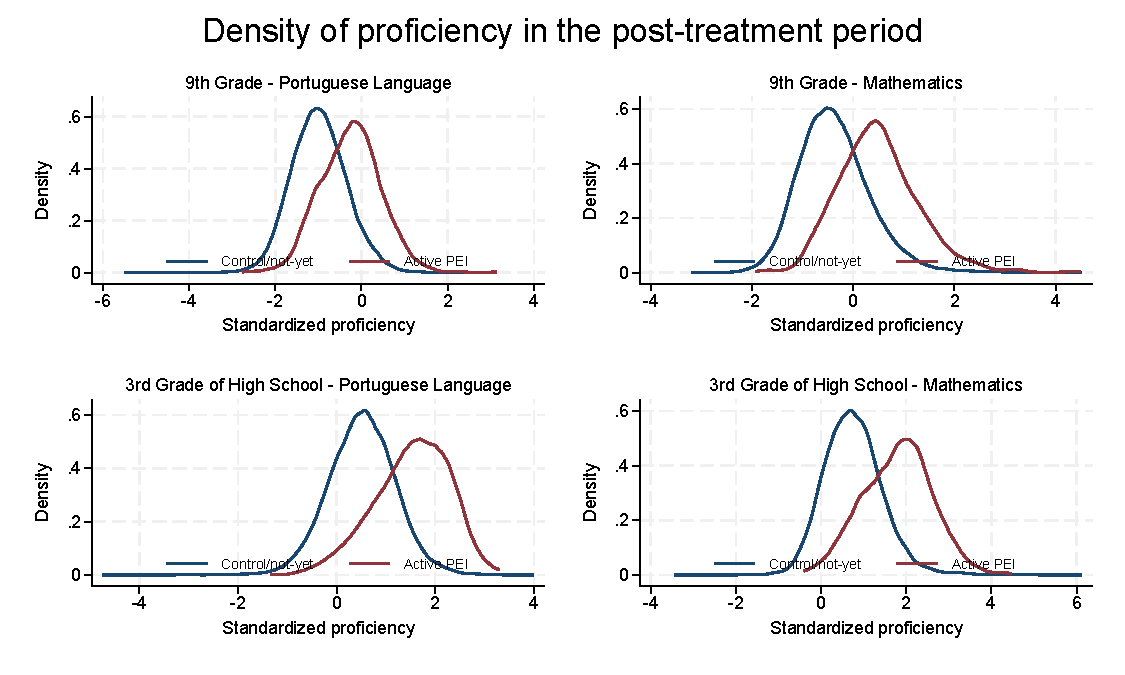
\includegraphics[width=0.95\textwidth]{files/images/densidade_medprof_pos_trat_controle.pdf}
    \caption{Density of proficiency in the post-treatment period}
    \label{fig:densidade_pos}
    \caption*{\footnotesize \textit{Source:} Author's elaboration. Treatment denotes school-year observations with active PEI; control denotes not-yet-treated or never-treated schools in the same calendar year.}
\end{figure}

In the aggregate panel, average proficiency in PEI schools increases by approximately 29 points in Portuguese Language and 30 points in Mathematics after conversion. The movement is large on the SARESP scale, but it still cannot be interpreted as causal. It shows that there is a relevant aggregate gain to be explained; the empirical question is how much of this gain remains when the comparison across schools is corrected.

\begin{table}[htbp]
\centering
\caption{Descriptive Statistics -- Aggregate Panel (School Level)}
\label{tab:agregado}
\small
\begin{threeparttable}
\begin{tabular}{lccccc}
\toprule
 & \multicolumn{3}{c}{Group Mean} & \multicolumn{2}{c}{Diff (Post--Pre)} \\
\cmidrule(lr){2-4} \cmidrule(lr){5-6}
Variable & Control & Treated Pre & Treated Post & Coef. & $p$-value \\
\midrule
Mean Proficiency, Portuguese & 243.8 & 244.7 & 273.5 & $+$28.8 & $<$0.001 \\
Mean Proficiency, Math       & 254.0 & 254.7 & 284.9 & $+$30.2 & $<$0.001 \\
Share Urban                  & 0.959 & 1.000 & 1.000 & --- & --- \\
Share Settlement             & 0.004 & 0.000 & 0.000 & --- & --- \\
\bottomrule
\end{tabular}
\begin{tablenotes}
\footnotesize
\item \textit{Note:} Proficiency is reported in the SARESP scale. ``---'' indicates no variation in the treated group for the respective characteristic.
\end{tablenotes}
\end{threeparttable}
\end{table}

\subsection{Main Results} \label{sec:resultadosprincipais}

Table \ref{tab:eventstudy_principal} presents the average post-treatment effect for each grade-subject combination. The reported number corresponds to the mean of coefficients from $k=0$ to $k=4$, with period $k=-1$ normalized as the common baseline.

\begin{table}[htbp]
\centering
\caption{Average post-treatment effect (standard deviations)}
\label{tab:eventstudy_principal}
\begin{tabular}{lcccc}
\toprule
Grade-subject & CS21 & DR-DiD & S\&X approx. & TWFE \\
\midrule
9th LP & \makecell{0.491***\\(0.019)} & \makecell{0.510***\\(0.019)} & \makecell{0.502***\\(0.028)} & \makecell{0.475***\\(0.017)} \\
9th Mat & \makecell{0.585***\\(0.020)} & \makecell{0.601***\\(0.020)} & \makecell{0.603***\\(0.033)} & \makecell{0.583***\\(0.018)} \\
HS3 LP & \makecell{0.526***\\(0.022)} & \makecell{0.571***\\(0.022)} & \makecell{0.601***\\(0.035)} & \makecell{0.507***\\(0.019)} \\
HS3 Mat & \makecell{0.605***\\(0.022)} & \makecell{0.627***\\(0.021)} & \makecell{0.675***\\(0.037)} & \makecell{0.604***\\(0.019)} \\
\bottomrule
\end{tabular}
\vspace{0.2cm}
\begin{flushleft}
\footnotesize Note: average from \(k=0\) to \(k=4\) of the event study with universal baseline at \(k=-1\), estimated in the 2011--2018 school-year-grade-subject panel. Conservative standard errors in parentheses, computed from the variances of period-specific coefficients; * \(p<0.10\), ** \(p<0.05\), *** \(p<0.01\).
\end{flushleft}
\end{table}





The full results by relative period, including standard errors for each estimator and grade-subject cell, are reported in Appendix~\ref{ap:principal}. This organization keeps the main text focused on the summary of average effects while preserving the complete estimation paths for inspection.

Effects are positive in all cells and for all estimators. In 9th grade, DR-DiD estimates an average effect of 0.510 standard deviations in Portuguese Language and 0.601 in Mathematics. The S\&X approximation produces very similar results: 0.502 and 0.603 standard deviations, respectively. In high school, effects are even larger. DR-DiD estimates 0.571 standard deviations in Portuguese Language and 0.627 in Mathematics; the S\&X approximation estimates 0.601 and 0.675.

The magnitude is substantive. Since the average annual standard deviation of proficiency in the panel is on the order of several dozen SARESP points, effects between approximately 0.50 and 0.68 standard deviations represent large shifts within the distribution of school performance. Reading the results in standard deviations should therefore not be seen as a statistical abstraction: it corresponds to relevant differences on the concrete exam scale.

These values are also high relative to the literature. Using linked data and focusing on São Paulo high schools, \textcite{scorzafave2023} estimate gains of 0.31 standard deviations in Mathematics and 0.21 in Portuguese Language. In Pernambuco, reported magnitudes for full-time schooling are around 0.20 standard deviations \parencite{Pernambuco}. This difference should not automatically be interpreted as evidence that the pedagogical effect estimated here is larger. This paper uses an aggregate school panel, annual standardization, its own window and sample, and does not directly observe the student-score link. For this reason, the main magnitudes should be read as aggregate evidence of gains associated with PEI and as potentially sensitive to the unit of analysis, SARESP participation, control-group composition, and covariate coverage.

The central point of the table is the relative stability of the estimates. Moving from CS21 to DR-DiD, which incorporates baseline proficiency, municipal controls, and aggregate composition covariates, does not eliminate the effect. Incorporating the S\&X approximation, now estimated only with four-category multinomial logits and without a binary fallback, also does not reduce the magnitude of the results. In high school, the S\&X estimate is even larger than the DR-DiD estimate, especially in Mathematics. Conservative variances and the small number of cells prevent precise inference about this difference; the available evidence is consistent with stability between DR-DiD and S\&X, but it cannot rule out smaller compositional effects.

TWFE appears with similar magnitudes, but should be read only as a reference. The policy has staggered adoption and effects grow with time since conversion. In this context, TWFE may combine inappropriate comparisons between already-treated schools and schools treated later. The main interpretation of the paper relies on CS21, DR-DiD, and the S\&X approximation, always conditional on the identification assumptions discussed in Section \ref{sec:methodsanddata}.

\subsection{Effect Dynamics} \label{sec:dinamicaefeito}

Figures \ref{fig:event_9ef_lp}--\ref{fig:event_em3_mat} show the trajectory of event-study coefficients. In general, effects appear in the year of conversion and grow in subsequent years. This pattern could reflect dynamic student selection, changes in exam participation, or recovery among schools initially below the mean; it is also compatible with a policy that takes time to reorganize pedagogical practices, school management, teacher dedication, and the use of the extended school day. Because these channels cannot be separated with the available data, the dynamics should be read as temporal evidence of the estimated aggregate effect, not as a direct test of mechanisms.

\begin{figure}[htbp]
    \centering
    \caption{9th Grade - Portuguese Language}
    \label{fig:event_9ef_lp}
    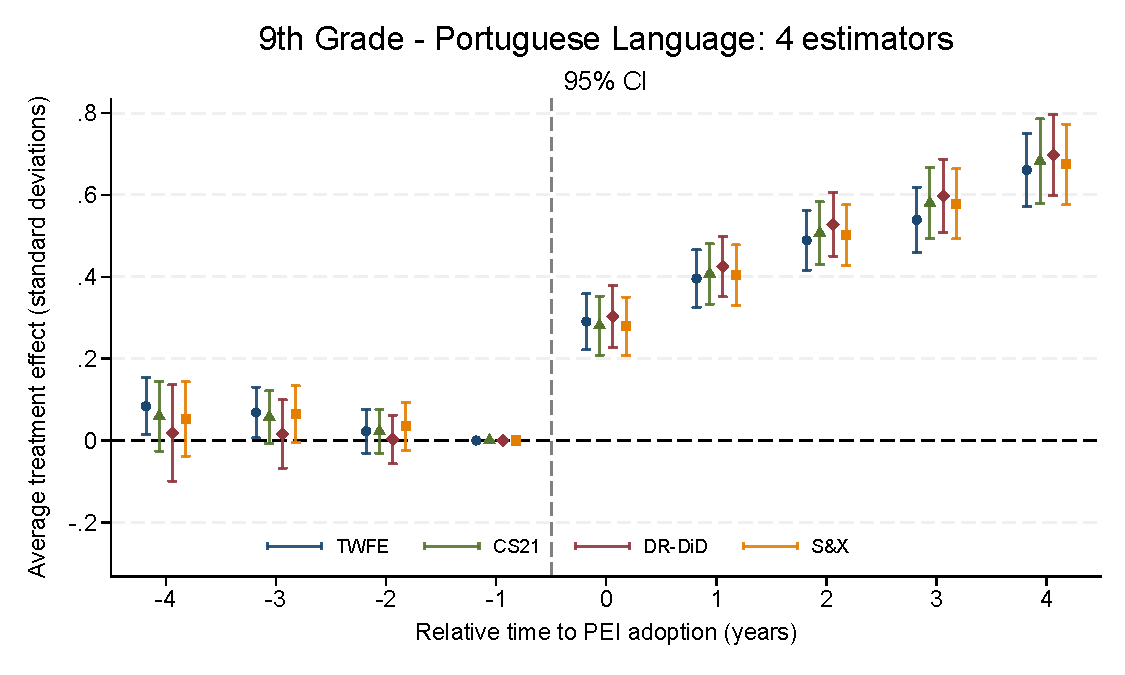
\includegraphics[width=0.95\textwidth]{files/images/eventstudy_all_9EF_LP.pdf}
    \caption*{\footnotesize \textit{Source:} author's elaboration. ATT coefficients by relative time to conversion; $k=0$ is the year of PEI adoption and $k=-1$ is the normalized baseline period. Bands indicate 95\% confidence intervals.}
\end{figure}

\begin{figure}[htbp]
    \centering
    \caption{9th Grade - Mathematics}
    \label{fig:event_9ef_mat}
    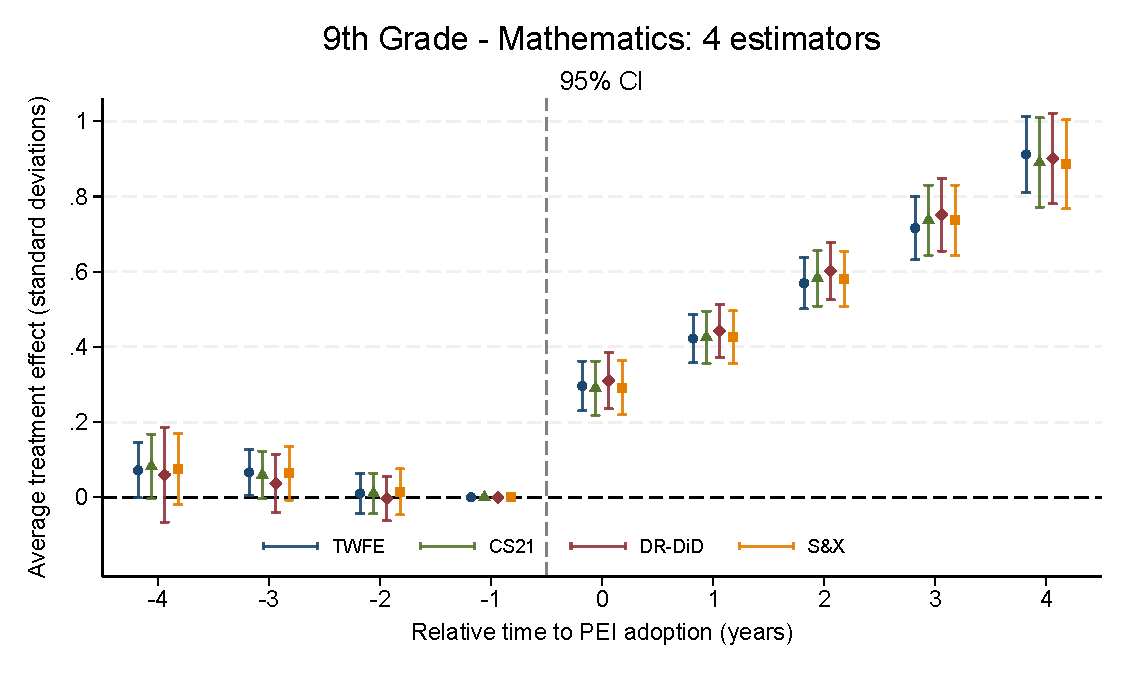
\includegraphics[width=0.95\textwidth]{files/images/eventstudy_all_9EF_Mat.pdf}
    \caption*{\footnotesize \textit{Source:} author's elaboration. ATT coefficients by relative time to conversion; $k=0$ is the year of PEI adoption and $k=-1$ is the normalized baseline period. Bands indicate 95\% confidence intervals.}
\end{figure}

\begin{figure}[htbp]
    \centering
    \caption{3rd Grade of High School - Portuguese Language}
    \label{fig:event_em3_lp}
    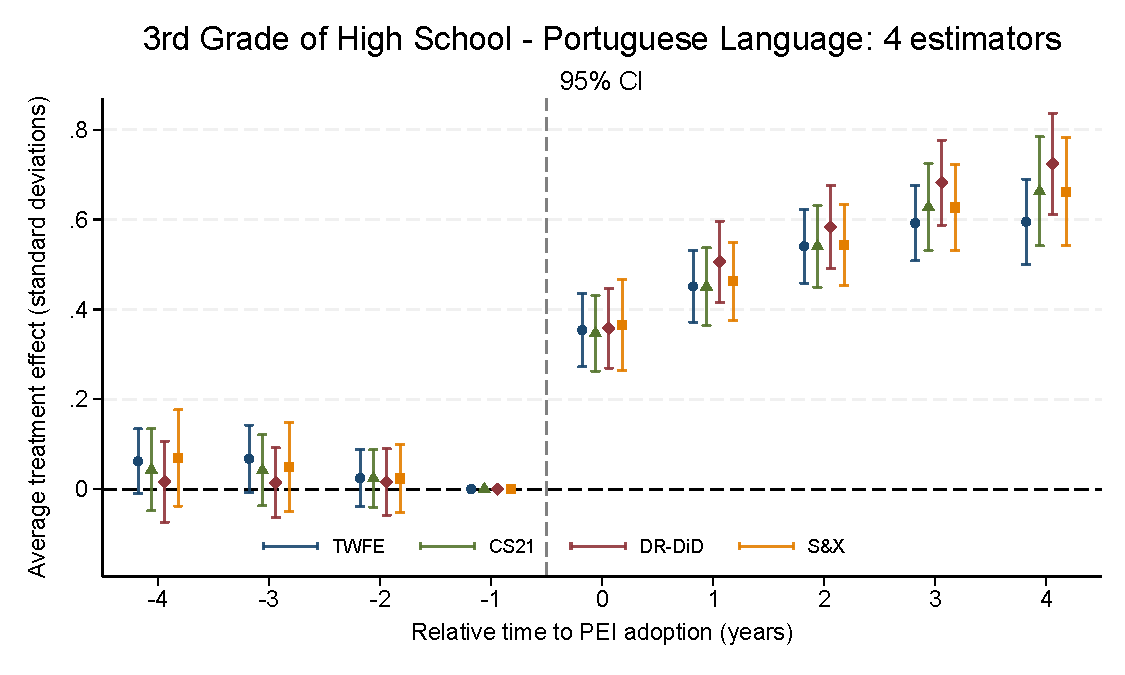
\includegraphics[width=0.95\textwidth]{files/images/eventstudy_all_EM3_LP.pdf}
    \caption*{\footnotesize \textit{Source:} author's elaboration. ATT coefficients by relative time to conversion; $k=0$ is the year of PEI adoption and $k=-1$ is the normalized baseline period. Bands indicate 95\% confidence intervals.}
\end{figure}

\begin{figure}[htbp]
    \centering
    \caption{3rd Grade of High School - Mathematics}
    \label{fig:event_em3_mat}
    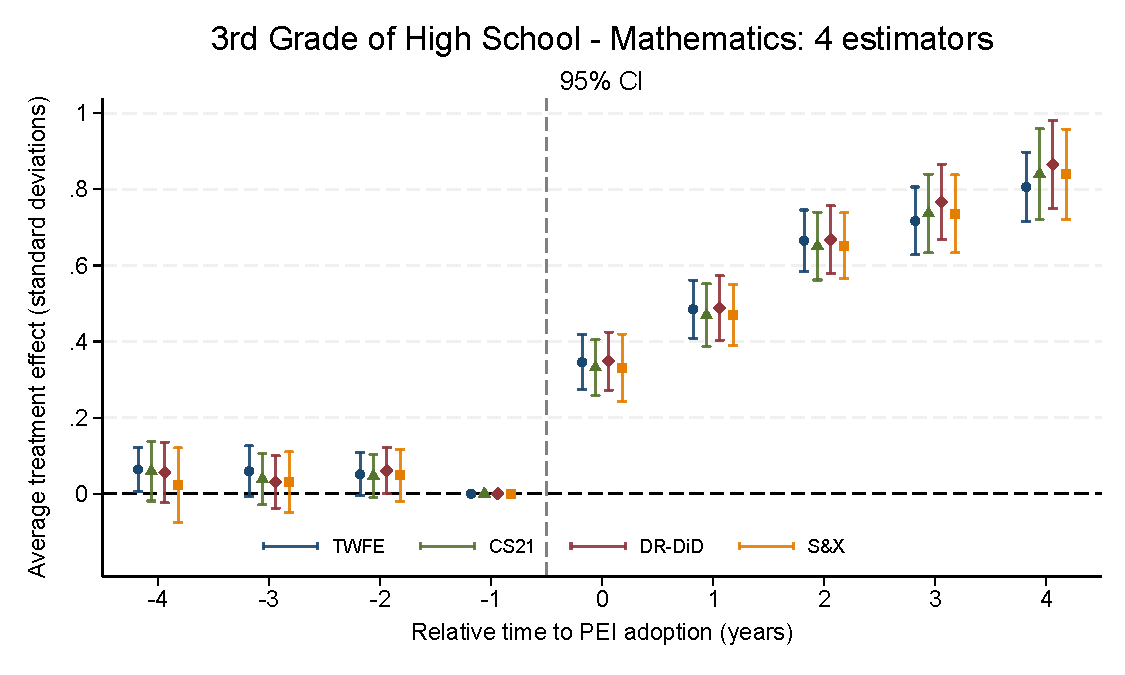
\includegraphics[width=0.95\textwidth]{files/images/eventstudy_all_EM3_Mat.pdf}
    \caption*{\footnotesize \textit{Source:} author's elaboration. ATT coefficients by relative time to conversion; $k=0$ is the year of PEI adoption and $k=-1$ is the normalized baseline period. Bands indicate 95\% confidence intervals.}
\end{figure}

Pre-treatment coefficients are smaller than post-treatment effects and, in the preferred specifications, do not form a systematic anticipation pattern. There are isolated differences in some cells, which is expected in an exercise with multiple grades, subjects, and estimators. Still, the main dynamic is clear: estimated post-treatment effects are positive, persistent, and increasing. This reading does not eliminate concern about mean reversion: pre-treatment balance shows that schools that would later join PEI had lower performance, especially in Mathematics, so part of the observed growth could reflect mechanical convergence. The baseline-support diagnostic below reduces, but does not eliminate, this threat.

The dynamics suggest stronger effects in Mathematics than in Portuguese Language. This difference should be interpreted as descriptive heterogeneity by subject, not as a definitive test of mechanisms. The available data do not allow me to distinguish whether the difference comes from learning, student selection, exam participation, or a combination of these channels.

\subsection{Composition and Robustness} \label{sec:robustez}

The central concern of the paper is that part of the observed gain in PEI schools may be generated by compositional change. Before looking at p-values, it is important to qualify the diagnostic: the comparison between DR-DiD and the S\&X approximation uses only 24 to 26 valid cells by grade-subject and adopts a conservative variance equal to the sum of marginal variances. Therefore, the test has low power to detect small or moderate differences. Table \ref{tab:hausman_composicao} presents this comparison and also reports the minimum detectable effect with 80\% power.

\begin{table}[htbp]
\centering
\caption{Hausman-type diagnostic: DR-DiD versus S\&X approximation}
\label{tab:hausman_composicao}
\small
\begin{threeparttable}
\begin{tabular}{lccccc}
\toprule
Grade-subject & DR-DiD & S\&X approx. & Diff. & \(p\)-value & MDE 80\% \\
\midrule
9th grade -- LP & 0.510 & 0.502 & -0.008 & 0.9630 & 0.198 \\
9th grade -- Mathematics & 0.601 & 0.603 & +0.002 & 0.9976 & 0.219 \\
HS3 -- LP & 0.571 & 0.601 & +0.031 & 0.9000 & 0.248 \\
HS3 -- Mathematics & 0.627 & 0.675 & +0.048 & 0.9057 & 0.243 \\
\bottomrule
\end{tabular}
\begin{tablenotes}
\footnotesize
\item \textit{Note:} DR-DiD and S\&X values correspond to the average post-treatment effect, computed as the mean from \(k=0\) to \(k=4\). The test uses a conservative variance equal to the sum of marginal variances. The 80\% MDE is the minimum detectable difference, in standard deviations, with 80\% power and a two-sided 5\% test. The S\&X approximation excludes cells without sufficient common support and does not use a binary DR-DiD fallback.
\end{tablenotes}
\end{threeparttable}
\end{table}





The p-values are high in all cells, but the minimum detectable difference ranges from 0.198 to 0.248 standard deviations. The correct reading is therefore restricted: given the available aggregate covariates and the conservative variance used in the test, there is no evidence that the compositional approximation produces statistically different effects from DR-DiD, but the test does not rule out differences smaller than approximately 0.20--0.25 standard deviations. Nor does it prove the absence of student selection, or replace an individual-level estimator with perfectly linked microdata. The p-values should be read as a sensitivity diagnostic, not as strong confirmation of compositional robustness.

It is also important to note what the S\&X approximation was actually able to estimate. In 9th grade, there were 26 valid cells per subject. In high school, there were 24. Excluded cells were not replaced by another estimator: they were removed because of insufficient common support in the multinomial logit. This point matters because it avoids reporting as S\&X an estimate that, in practice, would merely be binary DR-DiD in a subsample.

Table \ref{tab:diagnostico_regressao_media} presents a diagnostic for mean reversion. The baseline-support column re-estimates DR-DiD restricting the sample to the interval between the 10th and 90th percentiles of baseline proficiency among treated schools. This restriction forces the comparison to occur in a region of the distribution closer to the schools that joined PEI.

\begin{table}[htbp]
\centering
\caption{Mean-reversion diagnostic}
\label{tab:diagnostico_regressao_media}
\small
\begin{threeparttable}
\resizebox{\textwidth}{!}{%
\begin{tabular}{lcccc}
\toprule
Grade-subject & Main DR-DiD & Baseline support & $\Delta$ low controls & $\Delta$ high controls \\
\midrule
9th LP & 0.510 & 0.533 & 0.239 & -0.182 \\
9th Mat & 0.601 & 0.612 & -0.172 & -0.482 \\
HS3 LP & 0.571 & 0.581 & -0.094 & -0.578 \\
HS3 Mat & 0.627 & 0.607 & -0.295 & -0.542 \\
\bottomrule
\end{tabular}
}
\begin{tablenotes}
\footnotesize
\item \textit{Note:} The baseline-support column re-estimates DR-DiD restricting the sample to the p10--p90 interval of baseline proficiency among treated schools. The last two columns show the average change, in standard deviations, between 2011 and 2018 for never-treated controls below/above the treated-school baseline median.
\end{tablenotes}
\end{threeparttable}
\end{table}





The results change little relative to the main specification. In 9th grade, the Portuguese Language effect moves from 0.510 to 0.533 standard deviations and the Mathematics effect from 0.601 to 0.612. In high school, Portuguese Language moves from 0.571 to 0.581, while Mathematics moves from 0.627 to 0.607. This exercise does not fully eliminate the possibility of mean reversion, but it reduces the concern that the results are driven only by comparisons between initially weak treated schools and very distant controls at baseline. The last two columns also show that never-treated controls with low initial performance do not display a mechanical recovery capable of reproducing the magnitude of the estimated PEI effects.

Table \ref{tab:spillover_regional} evaluates the sensitivity of the results to possible regional contamination of the control group. The first restriction removes controls in school districts that already had at least one active PEI school in the year; the second uses a finer unit, the school-district-by-neighborhood pair.

\begin{table}[htbp]
\centering
\caption{Regional spillover diagnostic}
\label{tab:spillover_regional}
\begin{tabular}{llccc}
\toprule
Grade-subject & Restriction & Main DR-DiD & Restricted DR-DiD & Restricted N \\
\midrule
9th LP & DE & 0.510 & 0.482 & 13.739 \\
9th LP & DISTR & 0.510 & 0.526 & 21.097 \\
9th Mat & DE & 0.601 & 0.577 & 13.743 \\
9th Mat & DISTR & 0.601 & 0.615 & 21.107 \\
HS3 LP & DE & 0.571 & 0.563 & 13.221 \\
HS3 LP & DISTR & 0.571 & 0.571 & 20.947 \\
HS3 Mat & DE & 0.627 & 0.654 & 13.228 \\
HS3 Mat & DISTR & 0.627 & 0.634 & 20.959 \\
\bottomrule
\end{tabular}
\vspace{0.2cm}
\begin{flushleft}
\footnotesize Note: the restriction removes controls located in school districts (DE) or DE-neighborhood pairs (DISTR) that already had at least one active PEI school in the year. The estimator is DR-DiD; standard errors are omitted to keep the table compact. This is a regional proxy for spillover contamination of the counterfactual, not a measure of geographic distance.
\end{flushleft}
\end{table}





The estimates remain positive and close to the main estimates. Excluding controls by school district moderately reduces effects in 9th grade, from 0.510 to 0.482 in Portuguese Language and from 0.601 to 0.577 in Mathematics, but does not change the qualitative conclusion. In high school, effects also remain close. The school-district-by-neighborhood restriction is even more stable. Because this approach uses administrative proximity rather than geographic distance between schools, it should be read as a partial spillover diagnostic, not as a definitive solution for this channel. School districts may cover broad areas, while the mechanism documented by \textcite{santos2022_spillover_pei_escolas_regulares} operates through effective proximity between schools and student migration.

Table \ref{tab:robustez_sem_imputacao} presents a sensitivity diagnostic to imputation, repeating DR-DiD with complete raw covariates and no annual-mean imputation.

\begin{table}[htbp]
\centering
\caption{Sensitivity to covariate imputation}
\label{tab:robustez_sem_imputacao}
\resizebox{\textwidth}{!}{%
\begin{tabular}{lccccc}
\toprule
Grade-subject & DR-DiD (main) & DR-DiD no imputation & Main N & No-imputation N & N fraction \\
\midrule
9th LP & 0.510 & 0.384 & 24754 & 10804 & 0.436 \\
9th Mat & 0.601 & 0.502 & 24769 & 10819 & 0.437 \\
HS3 LP & 0.571 & -- & 27515 & -- & -- \\
HS3 Mat & 0.627 & -- & 27530 & -- & -- \\
\bottomrule
\end{tabular}
}
\vspace{0.2cm}
\begin{flushleft}
\footnotesize Note: the no-imputation version uses only observations with complete raw covariates. The exercise should be read as a diagnostic of sensitivity and sample coverage, not as a direct substitute for the main specification.
\end{flushleft}
\end{table}





The diagnostic reveals an important tension. Requiring complete covariates reduces the 9th-grade sample to about 44\% of the main sample and makes estimation infeasible in high school. In the two cells where estimation runs, effects remain positive, but fall to 0.384 standard deviations in Portuguese Language and 0.502 in Mathematics. This exercise does not replace the main specification, because it changes the sample composition; its function is to show that missing covariate data are empirically relevant and that annual-mean imputation preserves broader coverage of the state network.

\begin{table}[htbp]
\centering
\caption{Diagnostic of imputed covariates}
\label{tab:diagnostico_imputacao}
\begin{tabular}{lcccc}
\toprule
Grade-subject & Complete N & Imputed N & Complete baseline & Imputed baseline \\
\midrule
9th LP & 13.992 & 15.487 & 230.07 & 229,75 \\
9th Mat & 13.999 & 15.495 & 246,56 & 245,87 \\
HS3 LP & 1.032 & 27.842 & 266,68 & 265,49 \\
HS3 Mat & 1.033 & 27.857 & 272,48 & 269,72 \\
\bottomrule
\end{tabular}
\vspace{0.2cm}
\begin{flushleft}
\footnotesize Note: complete observations have all raw covariates used in the no-imputation DR-DiD. Baseline differences across columns indicate that the no-imputation diagnostic also changes sample composition. Baseline is mean proficiency on the SARESP scale.
\end{flushleft}
\end{table}





Table \ref{tab:diagnostico_imputacao} helps interpret this decline. In 9th grade, complete and imputed observations have very similar baseline proficiency, but the complete sample contains a smaller share of treated schools. In high school, the contrast is more severe: there are just over one thousand complete observations against almost 28 thousand with at least one imputed covariate, and the treated share in the complete sample is about one third of the share observed among imputed observations. Therefore, the no-imputation specification is better interpreted as a diagnostic of sensitivity and data coverage, not as a direct substitute for the main specification. In high school, the no-imputation column is empty because the loss of coverage prevents comparable estimation.

Taken together, the results indicate persistent gains associated with PEI adoption at the aggregate level, although the magnitude should be interpreted cautiously given the sensitivity to the no-imputation sample, the decline in SARESP participation in high school, and the limitations of the compositional test. The evidence is stronger for the question the data can answer: schools converted to the full-time model experience average proficiency gains relative to comparable schools within the 2011--2018 window. The evidence is more limited for the question that would require fully integrated microdata: how much of this gain comes exclusively from individual learning, net of all selection and changes in exam participation. This distinction is the empirical frontier of the paper. The exercise shows that observable aggregate composition does not eliminate the results, but it also makes clear that a complete individual decomposition remains beyond the reach of the available data.
